\documentclass{exam}

\usepackage{ctex}
\usepackage{amsmath}
\usepackage{physics}
\usepackage{anyfontsize}
\usepackage{bm}
\usepackage{tikz}

\renewcommand{\thequestion}{\zhnum{question}}
\renewcommand{\questionlabel}{\thequestion .}
\renewcommand{\thepartno}{\arabic{partno}}
\renewcommand{\partlabel}{\thepartno .}

\author{朱江云(整理)}
\title{电动力学第五章测验}
\date{}

\begin{document}
\maketitle
\begin{questions}
    \question 左旋圆偏振的单色平面电磁波自空气入射到电介质平面上,
    入射角为$\theta_1$,电介质的介电常数为$\epsilon$,磁导率为$\mu_0$。
    入射波的电场强度为
    \begin{equation*}
        \bm{E}(\bm{r},t) = E_0(\bm{e_1}+i\bm{e_2})e^{i(\bm{k} \cdot \bm{r}-\omega t)}
    \end{equation*}
    式中$\bm{e_1}$和$\bm{e_2}$是垂直于波矢$\bm{k}$的两个单位矢量,
    且$\bm{e_1} \bot \bm{e_2}$,$\bm{e_1} \times \bm{e_2} = \bm{k}/k$,
    $|k| = \omega \sqrt{\epsilon_0 \mu_0}=\omega/c $
    \begin{parts}
        \part 试求反射波和折射波的电场强度
        \part  由所得出的电场强度分析反射波和折射波的偏振状态
        \footnote{电动力学题解(第三版)3.22}
    \end{parts}
    \question 一对平行的无限大理想导体板相距为$b$,电磁波在其间沿$z$方向传
    播,取$y$轴垂直于板面,求

    \tikzset{every picture/.style={line width=0.75pt}} %set default line width to 0.75pt        

    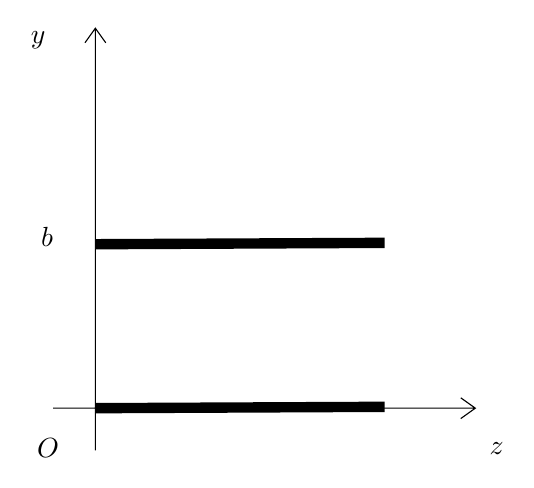
\begin{tikzpicture}[x=0.75pt,y=0.75pt,yscale=-1,xscale=1]
        %uncomment if require: \path (0,300); %set diagram left start at 0, and has height of 300

        %Shape: Axis 2D [id:dp6871113028816545] 
        \draw  (244,247.06) -- (447.4,247.06)(264.34,64) -- (264.34,267.4) (440.4,242.06) -- (447.4,247.06) -- (440.4,252.06) (259.34,71) -- (264.34,64) -- (269.34,71)  ;
        %Straight Lines [id:da8668350618290952] 
        \draw [line width=3.75]    (264.34,247.06) -- (403.67,246.4) ;
        %Straight Lines [id:da5302326625769478] 
        \draw [line width=3.75]    (264.34,168.06) -- (403.67,167.4) ;

        % Text Node
        \draw (453,262.4) node [anchor=north west][inner sep=0.75pt]    {$z$};
        % Text Node
        \draw (232,64.4) node [anchor=north west][inner sep=0.75pt]    {$y$};
        % Text Node
        \draw (237,158.4) node [anchor=north west][inner sep=0.75pt]    {$b$};
        % Text Node
        \draw (235,260.4) node [anchor=north west][inner sep=0.75pt]    {$O$};


    \end{tikzpicture}
    \begin{parts}
        \part 可能传播的TM型波的电磁场分布
        \part 波传播的截止频率和截止波长
        \part 波传播的相速度和群速度
        \part 分析能否传播TE、TEM型波
    \end{parts}
    \question 分别推导介质中和金属导体中的色散关系,并讨论二者的区别
\end{questions}
\end{document}